\chapter{RESULTS}
\label{ch:results}

This chapter is divided into two main sections. The first section focuses on the comparison of the two motion correction techniques. The second section focuses on the results of the machine learning algorithms applied to the metrics extracted from the images.

Each of the clinical images underwent volume registration using both registration methods outlined in Chapter \ref{ch:moco}. The FD and DVARs metrics were calculated for every pair of subsequent volumes $i$ and $i+1$ in the original sequences, the traditionally registered sequences, and the DAG-registered sequences. Then the sequences were comprehensively compared to themselves. For every volume in each sequence, the Dice metric, the mutual information, and the correlation ratio were calculated for the volume and every other volume in the sequence.

The simulated data underwent the same analyses as the clinical images, with one addition. Independent component analysis was performed on the simulated data to identify components contributing to the overall signal in the image. By correlating the components with the simulated signal for each image, the BOLD-related components were identifies. The amount of BOLD signal identified for each image was compared to that image's original BOLD signal.

To keep this chapter readable, tables and figures for results that did not have significant value have been moved to Appendix \ref{appendix:results}.

\section{Simulated Data}

\subsection{Volume Registration: Power Thresholds}

\begin{figure}[t]
	\centering
	\begin{subfigure}{0.4\textwidth}
		\centering
		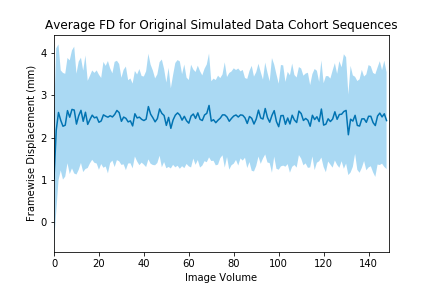
\includegraphics[width=1.0\textwidth]{6/figures/spectr-bold-fd-150.png}
		\caption{FD of Original Sequences.}
	\end{subfigure}
	\hspace{0.05\textwidth}
	\begin{subfigure}{0.4\textwidth}
		\centering
		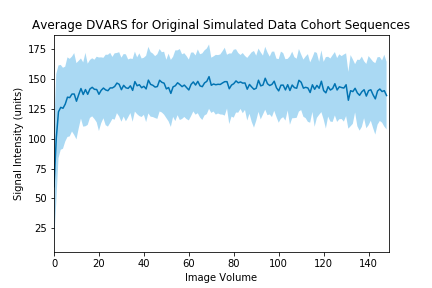
\includegraphics[width=1.0\textwidth]{6/figures/spectr-bold-dvars-150.png}
		\caption{DVARS of Original Sequences.}
	\end{subfigure}
	
	\begin{subfigure}{0.4\textwidth}
		\centering
		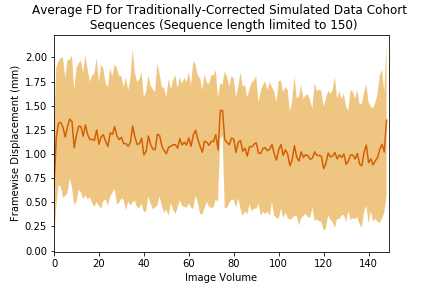
\includegraphics[width=1.0\textwidth]{6/figures/spectr-trad-fd-150.png}
		\caption{FD of Traditionally Registered Sequences.}
	\end{subfigure}
	\hspace{0.05\textwidth}
	\begin{subfigure}{0.4\textwidth}
		\centering
		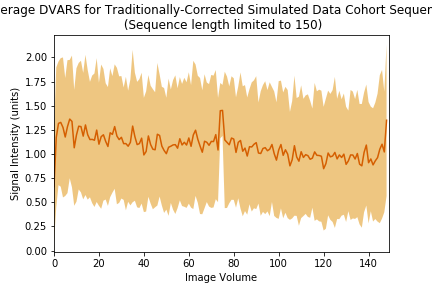
\includegraphics[width=1.0\textwidth]{6/figures/spectr-trad-dvars-150.png}
		\caption{DVARS of Traditionally Registered Sequences.}
	\end{subfigure}
	
	\begin{subfigure}{0.4\textwidth}
		\centering
		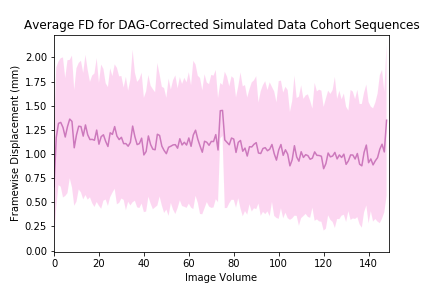
\includegraphics[width=1.0\textwidth]{6/figures/spectr-dag-fd-150.png}
		\caption{FD of DAG-Registered Sequences.}
	\end{subfigure}
	\hspace{0.05\textwidth}
	\begin{subfigure}{0.4\textwidth}
		\centering
		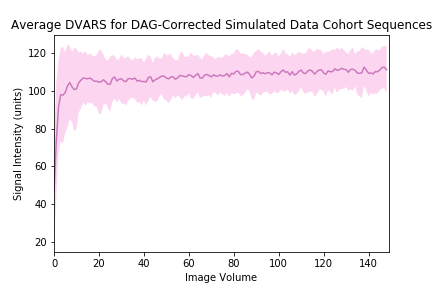
\includegraphics[width=1.0\textwidth]{6/figures/spectr-dag-dvars-150.png}
		\caption{DVARS of DAG-Registered Sequences.}
	\end{subfigure}
\caption{The means and standard deviations of the FD and DVARS metrics for all simulated images both before and after registration.}
\label{fig:spectr-power-dists}
\end{figure}

The FD and DVARS metrics were calculated between every pair of image volumes $i-1$ and $i$ for the original sequences and both types of registered sequences. The mean and standard deviation of the FD and DVARS metrics for each time point for each sequence type  can be seen in Figure \ref{fig:spectr-power-dists}. The mean of the FD metrics decreased from 2.45 mm in the original sequences to 1.07mm  and 1.08 mm in the traditionally and DAG-registered sequences. The standard deviations of the FD slightly increased from 0.084 mm in the original sequences to 0.265 mm and 0.173 mm, respectively. Similarly, the mean DVARS of the original sequences decreased from 141.67 units to 107.30 units and 107.15 units in the registered images. The standard deviation of the DVARS also increased from 3.66 units in the original sequences to 4.77 units and 4.73 units in the registered sequences.

\begin{table}[]
\centering
\caption{The number and percentage of image volumes across all sequences in the simulated cohort which meet the usability thresholds of FD \textless 0.2 mm and DVARS \textless 2.5\%.}
\label{tab:spectr-power-thresh}
\begin{tabular}{|c|c|c|c|}
\hline
\textbf{Threshold Met} &
  \textbf{\begin{tabular}[c]{@{}c@{}}Original\\  Sequences\end{tabular}} &
  \textbf{\begin{tabular}[c]{@{}c@{}}Traditionally Registered \\ Sequences\end{tabular}} &
  \textbf{\begin{tabular}[c]{@{}c@{}}DAG-Registered \\ Sequences\end{tabular}} \\ \hline
FD (count)    & 98    & 329   & 279   \\ \hline
DVARS (count) & 54    & 53    & 53    \\ \hline
Both (count)  & 53    & 46    & 44    \\ \hline
FD (\%)       & 0.731 & 2.453 & 2.081 \\ \hline
DVARS(\%)     & 0.403 & 0.395 & 0.395 \\ \hline
Both (\%)     & 0.395 & 0.343 & 0.328 \\ \hline
\end{tabular}
\end{table}

The FD and DVARS metrics for each image volume were compared to the usability criteria thresholds to determine the number of image volumes which were recovered by each registration type. The number of image volumes meeting the FD threshold, the DVARS threshold, and both thresholds were calculated. Table \ref{tab:spectr-power-thresh} shows the number of and percentage of image volumes which meet the specified thresholds. Across all 90 image sequences, there were 150 image volumes per sequence. The total number of image volumes for the simulated data was 13,410 image volumes. In the original images, less than 1\% of the image volumes met the individual thresholds with only 0.395\% of image volumes meeting both thresholds. After either registration, over 2\% of the image volumes meet the FD threshold, though there was no significant change in the number of image volumes meeting the DVARS threshold.

To determine the statistical significance of the differences in the number of image volumes meeting each threshold, a series of independent 2 sample t-tests were performed. For each test, two types of sequences were chosen. The distributions of samples were the numbers of image volumes in each sequence meeting the usability threshold of interest. The null hypotheses for the t-tests were that the number of volumes meeting the threshold for each sequence type were the same and the alternative hypothesis was that this number was different. The complete set of results can be seen in Table \ref{tab:spectr-power-ttest}. The only statistically significant differences in usability counts were for the number of image volumes meeting the FD threshold. The numbers of registered image volumes meeting the FD threshold for both registration types were significantly different from the counts for the original image sequences at $p < 0.005$. The difference between the two registration types was not significant ($p = 0.127$).

The distributions of the FD and DVARS metrics underwent pairwise comparison via sequence type for each subject. The pairwise comparisons were performed using the Kolmogorov-Smirnov test. The Kolmogorov-Smirnov test evaluates the difference between a pair of probability distributions. The FD and DVARS distributions were significantly different between the original and traditionally registered sequences and the original and DAG-registered sequences at $p < 0.005$. Between the traditionally registered and DAG-registered sequences, 40 sequences (44.4\%) had different FD distributions at $p < 0.05$ and 27 sequences (30.0\%) had different FD at $p < 0.005$. The two types of registrations only had 3 sequences (3.33\%) with different DVARS distributions at $p < 0.05$. This information can be found in table format in Tables \ref{tab:spectr-fd-kstest} and \ref{tab:spectr-dvars-kstest}.

Overall, the primary finding in the comparison of the registration techniques for the simulated data is the statistically significant decrease in FD by both registration types. There was also a decrease in the DVARS values for both registration types, but not a statistically significant one.

\subsection{Volume Registration: Sequence Duration Motion}

\begin{figure}
\centering
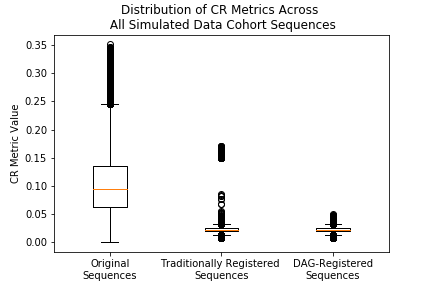
\includegraphics[height=0.3\textheight]{6/figures/spectr-cr-box.png}
\caption{Boxplots of the values of all CR matrices for the original sequences, the traditionally registered sequences, and the DAG-registered sequences for the simulated data.}
\label{fig:spectr-cr-box}
\end{figure}

\begin{figure}
\centering
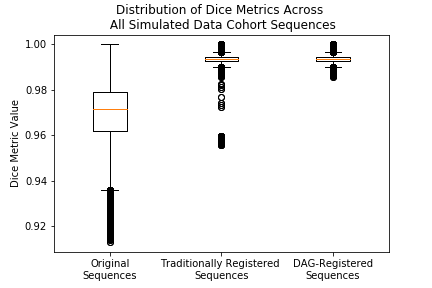
\includegraphics[height=0.3\textheight]{6/figures/spectr-dice-box.png}
\caption{Boxplots of the values of all Dice matrices for the original sequences, the traditionally registered sequences, and the DAG-registered sequences for the simulated data.}
\label{fig:spectr-dice-box}
\end{figure}

\begin{figure}
\centering
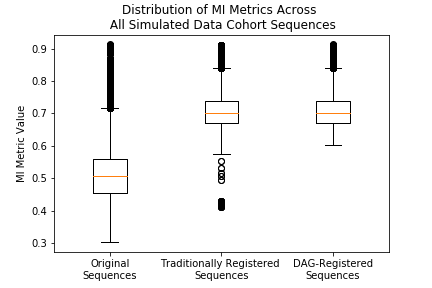
\includegraphics[height=0.3\textheight]{6/figures/spectr-mi-box.png}
\caption{Boxplots of the values of all MI matrices for the original sequences, the traditionally registered sequences, and the DAG-registered sequences for the simulated data.}
\label{fig:spectr-mi-box}
\end{figure}


The FD and DVARS metrics measure motion with respect to an pair of usability standards, but they offer a limited perspective about the motion present throughout an image sequence. Motion across the entire image was measured by calculating a similarity metric between every image volume $i$ and every other image volume $j$. The 

Motion across the whole sequence was measured by comparing every image volume in the sequence to every other image volume in the sequence. The three metrics used for this comparison were the correlation ratio (CR), the Dice metric, and mutual information (MI). The calculations for a single metric on one sequence produce a two dimensional matrix of metric values. 

These matrices were used to compare the quantities of motion over the course of an entire sequence. 

Box and whisker plots show the distributions of the metrics across the simulated data cohort for the correlation ratio matrices, the Dice matrices, and the mutual information matrices in Figures \ref{fig:spectr-cr-box}, \ref{fig:spectr-dice-box}, and \ref{fig:spectr-mi-box}, respectively. To describe the distribution of the similarity metrics matrices for the original sequence and each registered sequence, the minimum, first quartile, median, third quartile, and maximum values of each matrix were computed. The distributions of these five values were compared between registration types using two sample t-tests. 

The t-tests showed that for the CR matrices, the original have statistically significantly different first quartiles, medians, third quartiles, and maximum values from the registered sequences at $p < 0.005$. The minimum values of the CR distributions were not significantly different. Similar minimum values in the CR distributions were expected: the CR measures the distance between a pair of distributions and the minimum distance has a low valued asymptote. The Dice metric and MI matrices showed similar statistical differences, though these metrics have upper bound instead of a lower bound. The original sequences have statistically significantly different minimums, first quartiles, medians, and third quartiles from the registered sequences at $p < 0.005$ and similar maximum values. The p-values for these calculations can be seen in Table \ref{tab:spectr-cr-ttest} for the correlation ratio matrices, Table \ref{tab:spectr-dice-ttest} for the Dice matrices, and Table \ref{tab:spectr-mi-ttest} for the MI matrices. 

The distributions of all matrix values for the same similarity metric were compared using the Kolmogorov-Smirnov test. Three Kolmogorov-Smirnov tests were performed for each metric type to compare the distributions for the original and traditionally registered sequences, the original and DAG-registered sequences, and the traditionally registered and DAG-registered sequences. The tests showed that each pair of distributions for each metric type differed with a statistical significance of $p < 0.005$.

The analysis of sequence level motion was performed using three metrics to measure the similarity of the volumes across each sequence. The matrices were compared to each other with respect to five descriptive statistics and with respect to the distribution of the entired set of s imilarity matrices for the original image sequences and each registration type. The distributions of the similarity metrics were found to be statistically significantly different, implying that each type of sequence contains different motion patterns.


\subsection{Volume Registration: Recovered Signal}

One of the benefits of creating simulated data is that the signal and noise added to each image is known. 

The registered images underwent independent component analysis (ICA) to identify signal components which contribute to the image as a whole. Traditionally, ICA is used to identify signal components correlated with patient motion so that they can be regressed out of the image sequence. Since the BOLD signal added to each simulated image is known, ICA can be used to determine how much BOLD signal is retained after volume registration.

ICA was applied to all registered sequences to identify the signal components. For each sequence, the components were compared to the DMN ROI. The components with the largest correlation to the DMN ROI were categorized as the BOLD-related components. The average correlations between the BOLD-related components and the DMN ROI were 8122.41 for the traditionally registered sequences and 8039.52 for the DAG-registered sequences. The correlations for the traditionally registered sequences and the DAG-registered sequences were compared using the Kolmogorov-Smirnov test and a two-sample t-test. Neither the test estimated a statistical significance between the correlation distributions for the registered sequences (KS p-value = 0.999; t-test p-value 0.807).

\begin{table}[]
\centering
\caption{The average true and false rates for both positive and negative voxels when comparing the IC component with the largest correlation to the DMN ROI over each simulated image.}
\label{tab:spectr-avg-rates}
\begin{tabular}{|c|c|c|}
\hline
\textbf{Average Value} & \textbf{Traditionally Registered} & \textbf{DAG-Registered} \\ \hline
TPR                    & 0.587                             & 0.623                   \\ \hline
FPR                    & 0.104                             & 0.00996                 \\ \hline
TNR                    & 0.990                             & 0.990                   \\ \hline
FNR                    & 0.413                             & 0.377                   \\ \hline
\end{tabular}
\end{table}

To determine the accuracy of the BOLD-related components, the component image volumes were compared to the DMN ROI on a voxel level. The absolute value of each component image volume was taken and thresholded at 10\% of the maximum absolute value. The thresholded component image volumes were compared to DMN ROI. The counts of voxels which were true positive, false positive, true negative, and false negative were calculated, where the DMN ROI was treated as the ground truth. The average true positive rates, false positive rates, true negative rates, and false negative rates for each registration type were calculated. These values can be seen in Table \ref{tab:spectr-avg-rates}. The rates were compared for the traditionally registered and DAG-registered sequences. While none of the rates were statistically significant at even $ p < 0.05$, the rates were better for the DAG-registered sequences than for the traditionally registered sequences. 

\section{Preadolescent Cohort}

\subsection{Volume Registration: Power Thresholds}

% First: FD and DVARs
The averages of the distributions of the FD and DVARs metrics across the whole time period of the sequences for the original, traditionally registered, and DAG-registered images were calculated. The images sequences varied in length from 150 volume to 450 volumes due to the differences in acquisition protocols at different sites. The means and standard deviations of FD and DVARS metrics for the entire set of sequence with their original lengths can be seen in Figures \ref{fig:pread-fd-450} and \ref{fig:pread-dvars-450}. The means and standard deviations of the FD and DVARs metrics for the first 150 volumes in each sequence can be seen in Figures \ref{fig:pread-dvars-150} and \ref{fig:pread-dvars-150}. 


To compare the FD and DVARS values for each type of motion correction, the metrics for each image were considered to be independent samples drawn from an unknown distribution. Pairwise comparisons of these distribution were performed using the Kolmogorov-Smirnov (KS) test. The two-sided KS test measures the distance between the empirical distributions of two distributions. The null hypothesis of the two-sided KS test is that the empirical distributions being compared come from the same underlying distribution. As the KS test is nonparametric, the metrics for all image volumes can be used.

By comparing the distributions for the original sequences to the distributions for the registered sequences, we aim to determine if the volume registration had a significant effect on the images themselves. The comparison of the distributions for the two types of registered images is intended to determine if there is a statistically significant difference between the FD and DVARS distributions of the registered images.


The KS statistic and p-value produced as result of the KS tests can be seen in Table \ref{tab:pread-ks-fd} for the FD metrics and in Table \ref{tab:pread-ks-dvars} for the DVARS metrics.


%Each rs-fMRI sequence in the cohort underwent registration using both frameworks. For each sequence, the correlation ratio between every possible pair of volumes was calculated. A set of metrics of the correlation ratio matrices for each sequence can be seen in Table \ref{tab:crm-stats}. This table shows that the original sequences generally have higher average correlation ratios and contain more variation in their correlation ratios than the globally registered images. The registration methods were able to reduce the mean and variability of the correlation ratios across all subjects in the cohort who had original correlation ratio averages of at least 0.035.



The FD and DVARS values were compared to the usability thresholds defined by Power et al. to determine how many volumes were recovered by each framework \cite{Power2014}. Table \ref{tab:pread-powerthresh} shows the number of volumes meeting each threshold, both in terms of the number of volumes in the cohort and the percentage of volumes in the cohort. In the original dataset, almost 42\% of image volumes met both the FD and DVARS thresholds. However, only about 5\% of volumes met both thresholds for each registration type. Looking at the thresholds independently, about 60\% of volumes met the FD threshold before registration and only 16\% of volumes met the threshold after registration. Similarly, about 48\% of volumes met the DVARS threshold before registration and only about 6\% of volumes met the threshold after registration. These results suggest that the registration process introduces some degree of error into the preadolescent images, at least with respect to the established usability criteria.

\begin{figure}[ht]
\centering
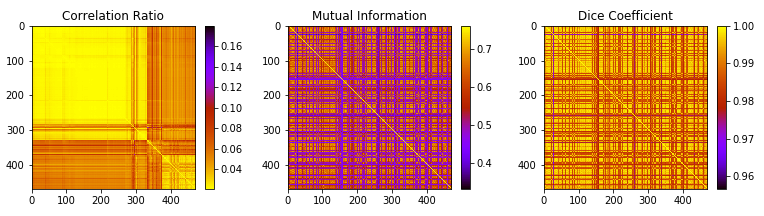
\includegraphics[width=1\textwidth]{6/figures/similarity-mat-sample.png}
\caption{Examples of the three similarity matrices. Lighter colors represent more desirable values.}
\label{fig:sim-mat-sample}
\end{figure}

An example of the three similarity matrices can be seen in Figure \ref{fig:sim-mat-sample}. The element $e_{i,j}$ represents the value of the given metric between the image volumes represented by row $i$ and column $j$. Each metric measures similarity according to slightly different definitions. In this figure, lighter values represent better metric values while darker values indicate lower similarity.

It is important to note the scales for these three metrics vary. The correlation ratio measures the distance between two items. Lower values for the correlation ratio means there is a smaller distance between the given pair of image volumes. The mutual information measures the shared information between two distributions of samples which may or may not be generated from the same underlying distribution. Higher mutual information values mean more shared information and low values mean less shared information. The Dice coefficient measures the overlap of two binary images. High Dice coefficients indicate a large amount of overlap, with a value of 1.0 indicating a perfect overlap.

The correlation ratio matrix in Figure \ref{fig:sim-mat-sample} suggests that the patient remained relatively still for the first 300 volumes of the image, then moved for about 100 volumes, and remained still in a new position for the last 50 frames of the sequence. The colors representing the correlation ratios correspond to very low values, suggesting there is little patient motion overall.

The Dice coefficient matrix has a similar pattern as the mutual information matrix, but leads to a different conclusion. The Dice coefficient was calculated on an Otsu thresholded version of each image volume. As the values of the Dice coefficients are consistently high, the patient likely did not move much. 

The mutual information matrix shows that the shared information throughout the entire image sequence varies. Using the information from the correlation ratio matrix and the Dice coefficient matrix, it is possible that the variations in the mutual information matrix are due to changes in the rs-fMRI signal caused by BOLD signal changes, spin history effects of motion, and susceptibility effects of motion.

\subsection{Volume Registration: Sequence Duration Motion}

\begin{figure}
\centering
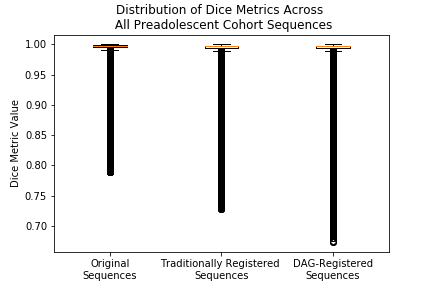
\includegraphics[width=0.5\textwidth]{6/figures/preads-dice-box.png}
\caption{Boxplots of the values of all Dice matrices for the original sequences, the traditionally registered sequences, and the DAG-registered sequences for the preadolescent cohort.}
\label{fig:preads-dice-box}
\end{figure}

\begin{figure}
\centering
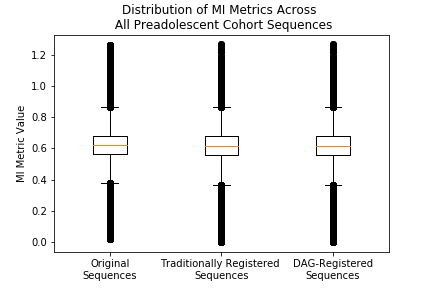
\includegraphics[width=0.5\textwidth]{6/figures/preads-mi-box.png}
\caption{Boxplots of the values of all MI matrices for the original sequences, the traditionally registered sequences, and the DAG-registered sequences for the preadolescent cohort.}
\label{fig:preads-mi-box}
\end{figure}

The distributions of the metrics matrices were compared to each other using the Kolmogorov-Smirnov test for each sequence type. The metrics for the Dice matrices and the mutual information matrices were determined to be from different distributions for each sequence type at p < 0.005.

\begin{table}[]
\centering
\caption{The number of preadolescent subjects whose sequences of types $S_1$ and $S_2$ had different MI distributions.}
\label{tab:preads-mi-kstest}
\begin{tabular}{|c|c|c|c|}
\hline
\textbf{\begin{tabular}[c]{@{}c@{}}\# Sequences \\ Type 1 ($S_1$)\end{tabular}} &
  \textbf{\begin{tabular}[c]{@{}c@{}}\# Sequences \\ Type 2 ($S_2$)\end{tabular}} &
  \textbf{\begin{tabular}[c]{@{}c@{}}\# Sequences \\ p \textless 0.05\end{tabular}} &
  \textbf{\begin{tabular}[c]{@{}c@{}}\# Sequences \\ p \textless 0.005\end{tabular}} \\ \hline
Original                                                            & \begin{tabular}[c]{@{}c@{}}Traditionally\\ Registered\end{tabular} & 189 & 187 \\ \hline
Original                                                            & \begin{tabular}[c]{@{}c@{}}DAG\\ Registered\end{tabular}           & 189 & 185 \\ \hline
\begin{tabular}[c]{@{}c@{}}Traditionally \\ Registered\end{tabular} & \begin{tabular}[c]{@{}c@{}}DAG\\ Registered\end{tabular}           & 84  & 69 \\ \hline
\end{tabular}
\end{table}

\begin{table}[]
\centering
\caption{The number of preadolescent subjects whose sequences of types $S_1$ and $S_2$ had different Dice distributions.}
\label{tab:preads-dice-kstest}
\begin{tabular}{|c|c|c|c|}
\hline
\textbf{\begin{tabular}[c]{@{}c@{}}\# Sequences \\ Type 1 ($S_1$)\end{tabular}} &
  \textbf{\begin{tabular}[c]{@{}c@{}}\# Sequences \\ Type 2 ($S_2$)\end{tabular}} &
  \textbf{\begin{tabular}[c]{@{}c@{}}\# Sequences \\ p \textless 0.05\end{tabular}} &
  \textbf{\begin{tabular}[c]{@{}c@{}}\# Sequences \\ p \textless 0.005\end{tabular}} \\ \hline
Original                                                            & \begin{tabular}[c]{@{}c@{}}Traditionally\\ Registered\end{tabular} & 188 & 185 \\ \hline
Original                                                            & \begin{tabular}[c]{@{}c@{}}DAG\\ Registered\end{tabular}           & 187 & 185 \\ \hline
\begin{tabular}[c]{@{}c@{}}Traditionally \\ Registered\end{tabular} & \begin{tabular}[c]{@{}c@{}}DAG\\ Registered\end{tabular}           & 83  & 75  \\ \hline
\end{tabular}
\end{table}

%-----------------------------------------------------------------
\section{Neonatal Cohort}

\subsection{Volume Registration: Power Thresholds}

\begin{figure}[t]
	\centering
	\begin{subfigure}{0.4\textwidth}
		\centering
		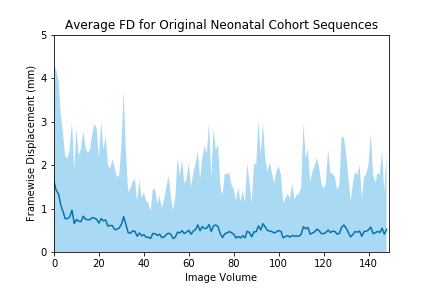
\includegraphics[width=1.0\textwidth]{6/figures/neonates-bold-fd-150.png}
		\caption{FD of Original Sequences.}
	\end{subfigure}
	\hspace{0.05\textwidth}
	\begin{subfigure}{0.4\textwidth}
		\centering
		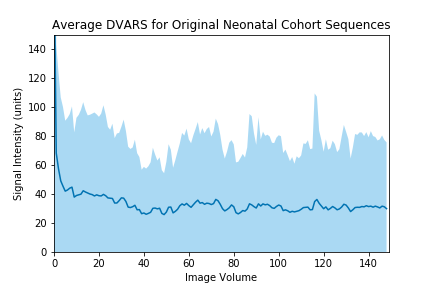
\includegraphics[width=1.0\textwidth]{6/figures/neonates-bold-dvars-150.png}
		\caption{DVARS of Original Sequences.}
	\end{subfigure}
	
	\begin{subfigure}{0.4\textwidth}
		\centering
		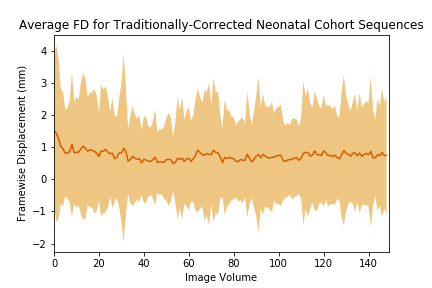
\includegraphics[width=1.0\textwidth]{6/figures/neonates-trad-fd-150.png}
		\caption{FD of Traditionally Registered Sequences.}
	\end{subfigure}
	\hspace{0.05\textwidth}
	\begin{subfigure}{0.4\textwidth}
		\centering
		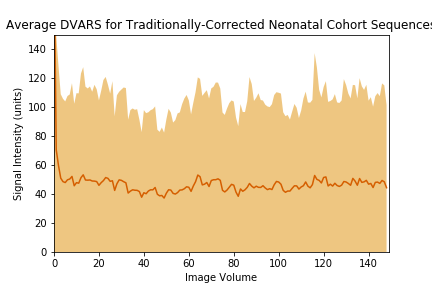
\includegraphics[width=1.0\textwidth]{6/figures/neonates-trad-dvars-150.png}
		\caption{DVARS of Traditionally Registered Sequences.}
	\end{subfigure}
	
	\begin{subfigure}{0.4\textwidth}
		\centering
		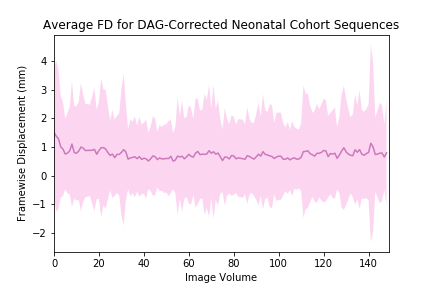
\includegraphics[width=1.0\textwidth]{6/figures/neonates-dag-fd-150.png}
		\caption{FD of DAG-Registered Sequences.}
	\end{subfigure}
	\hspace{0.05\textwidth}
	\begin{subfigure}{0.4\textwidth}
		\centering
		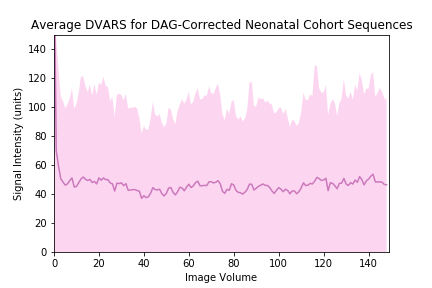
\includegraphics[width=1.0\textwidth]{6/figures/neonates-dag-dvars-150.png}
		\caption{DVARS of DAG-Registered Sequences.}
	\end{subfigure}
\caption{The means and standard deviations of the FD and DVARS metrics for all neonatal images both before and after registration.}
\label{fig:neonate-power-dists}
\end{figure}

\begin{table}[]
\centering
\caption{The number and percentage of image volumes across all sequences in the neonatal cohort which meet the usability thresholds of FD \textless 0.2 mm and DVARS \textless 2.5\%.}
\label{tab:neonate-power-thresh}
\begin{tabular}{|c|c|c|c|}
\hline
\textbf{Threshold Met} &
  \textbf{\begin{tabular}[c]{@{}c@{}}Original\\  Sequences\end{tabular}} &
  \textbf{\begin{tabular}[c]{@{}c@{}}Traditionally Registered \\ Sequences\end{tabular}} &
  \textbf{\begin{tabular}[c]{@{}c@{}}DAG-Registered \\ Sequences\end{tabular}} \\ \hline
FD (count)    & 16495  & 14264 & 14173 \\ \hline
DVARS (count) & 16820  & 13903 & 13752 \\ \hline
Both (count)  & 15332  & 12837 & 12684 \\ \hline
FD (\%)       & 69.59  & 60.18 & 59.79 \\ \hline
DVARS(\%)     & 70.96  & 58.65 & 58.02 \\ \hline
Both (\%)     & 64.68  & 54.16 & 53.51 \\ \hline
\end{tabular}
\end{table}

Table \ref{tab:neonate-power-thresh} contains the number and percentages of image volumes from the whole neonatal cohort which meet the FD and DVARS thresholds. The total number of image volumes in across all sequences of a single type was 23704.

\subsection{Volume Registration: Sequence Duration Motion}

\begin{figure}
\centering
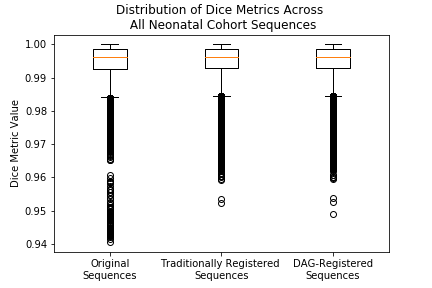
\includegraphics[width=0.5\textwidth]{6/figures/neonates-dice-box.png}
\caption{Boxplots of the values of all Dice matrices for the original sequences, the traditionally registered sequences, and the DAG-registered sequences for the neonatal cohort.}
\label{fig:neonates-dice-box}
\end{figure}

\begin{figure}
\centering
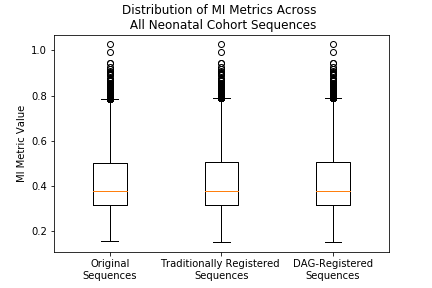
\includegraphics[width=0.5\textwidth]{6/figures/neonates-mi-box.png}
\caption{Boxplots of the values of all MI matrices for the original sequences, the traditionally registered sequences, and the DAG-registered sequences for the neonatal cohort.}
\label{fig:neonates-mi-box}
\end{figure}

The distributions of the metrics matrices were compared to each other using the Kolmogorov-Smirnov test for each sequence type. The metrics for the Dice matrices and the mutual information matrices were determined to be from different distributions for each sequence type at p < 0.005.

\begin{table}[]
\centering
\caption{The number of neonatal subjects whose sequences of types $S_1$ and $S_2$ had different MI distributions.}
\label{tab:neonates-mi-kstest}
\begin{tabular}{|c|c|c|c|}
\hline
\textbf{\begin{tabular}[c]{@{}c@{}}\# Sequences \\ Type 1 ($S_1$)\end{tabular}} &
  \textbf{\begin{tabular}[c]{@{}c@{}}\# Sequences \\ Type 2 ($S_2$)\end{tabular}} &
  \textbf{\begin{tabular}[c]{@{}c@{}}\# Sequences \\ p \textless 0.05\end{tabular}} &
  \textbf{\begin{tabular}[c]{@{}c@{}}\# Sequences \\ p \textless 0.005\end{tabular}} \\ \hline
Original                                                            & \begin{tabular}[c]{@{}c@{}}Traditionally\\ Registered\end{tabular} & 66 & 64 \\ \hline
Original                                                            & \begin{tabular}[c]{@{}c@{}}DAG\\ Registered\end{tabular}           & 71 & 69 \\ \hline
\begin{tabular}[c]{@{}c@{}}Traditionally \\ Registered\end{tabular} & \begin{tabular}[c]{@{}c@{}}DAG\\ Registered\end{tabular}           & 64 & 64  \\ \hline
\end{tabular}
\end{table}

\begin{table}[]
\centering
\caption{The number of neonatal subjects whose sequences of types $S_1$ and $S_2$ had different Dice distributions.}
\label{tab:neonates-dice-kstest}
\begin{tabular}{|c|c|c|c|}
\hline
\textbf{\begin{tabular}[c]{@{}c@{}}\# Sequences \\ Type 1 ($S_1$)\end{tabular}} &
  \textbf{\begin{tabular}[c]{@{}c@{}}\# Sequences \\ Type 2 ($S_2$)\end{tabular}} &
  \textbf{\begin{tabular}[c]{@{}c@{}}\# Sequences \\ p \textless 0.05\end{tabular}} &
  \textbf{\begin{tabular}[c]{@{}c@{}}\# Sequences \\ p \textless 0.005\end{tabular}} \\ \hline
Original                                                            & \begin{tabular}[c]{@{}c@{}}Traditionally\\ Registered\end{tabular} & 67 & 66 \\ \hline
Original                                                            & \begin{tabular}[c]{@{}c@{}}DAG\\ Registered\end{tabular}           & 71 & 69 \\ \hline
\begin{tabular}[c]{@{}c@{}}Traditionally \\ Registered\end{tabular} & \begin{tabular}[c]{@{}c@{}}DAG\\ Registered\end{tabular}           & 68 & 64  \\ \hline
\end{tabular}
\end{table}

\section{Fetal Cohort}

\subsection{Brain}

\subsubsection{Volume Registration: Power Thresholds}

\begin{figure}[t]
	\centering
	\begin{subfigure}{0.4\textwidth}
		\centering
		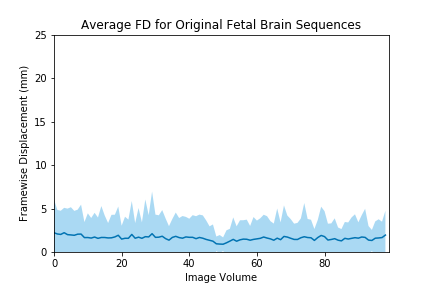
\includegraphics[width=1.0\textwidth]{6/figures/fetal-brain-bold-fd-150.png}
		\caption{FD of Original Sequences.}
	\end{subfigure}
	\hspace{0.05\textwidth}
	\begin{subfigure}{0.4\textwidth}
		\centering
		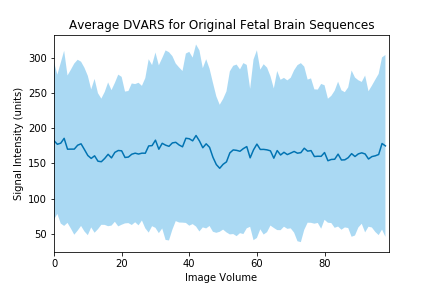
\includegraphics[width=1.0\textwidth]{6/figures/fetal-brain-bold-dvars-150.png}
		\caption{DVARS of Original Sequences.}
	\end{subfigure}
	
	\begin{subfigure}{0.4\textwidth}
		\centering
		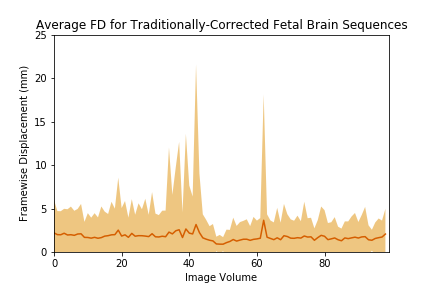
\includegraphics[width=1.0\textwidth]{6/figures/fetal-brain-trad-fd-150.png}
		\caption{FD of Traditionally Registered Sequences.}
	\end{subfigure}
	\hspace{0.05\textwidth}
	\begin{subfigure}{0.4\textwidth}
		\centering
		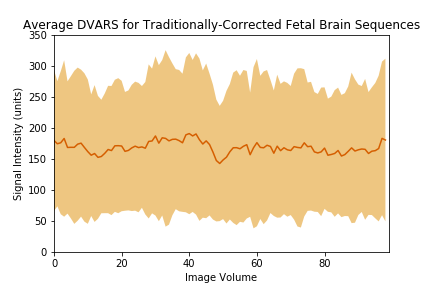
\includegraphics[width=1.0\textwidth]{6/figures/fetal-brain-trad-dvars-150.png}
		\caption{DVARS of Traditionally Registered Sequences.}
	\end{subfigure}
	
	\begin{subfigure}{0.4\textwidth}
		\centering
		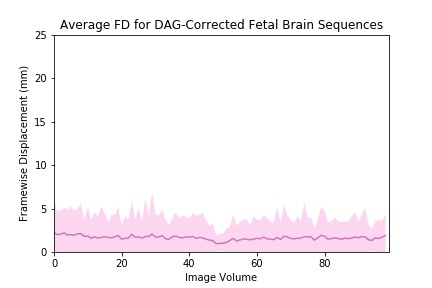
\includegraphics[width=1.0\textwidth]{6/figures/fetal-brain-dag-fd-150.png}
		\caption{FD of DAG-Registered Sequences.}
	\end{subfigure}
	\hspace{0.05\textwidth}
	\begin{subfigure}{0.4\textwidth}
		\centering
		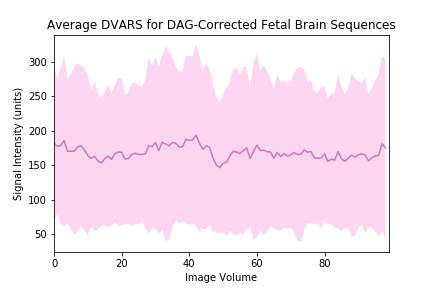
\includegraphics[width=1.0\textwidth]{6/figures/fetal-brain-dag-dvars-150.png}
		\caption{DVARS of DAG-Registered Sequences.}
	\end{subfigure}
\caption{The means and standard deviations of the FD and DVARS metrics for all fetal brain images both before and after registration.}
\label{fig:fetal-brain-power-dists}
\end{figure}

\begin{table}[]
\centering
\caption{The number and percentage of image volumes across all sequences in the fetal brain image data set which meet the usability thresholds of FD \textless 0.2 mm and DVARS \textless 2.5\%.}
\label{tab:fetal-brain-power-thresh}
\begin{tabular}{|c|c|c|c|}
\hline
\textbf{Threshold Met} &
  \textbf{\begin{tabular}[c]{@{}c@{}}Original\\  Sequences\end{tabular}} &
  \textbf{\begin{tabular}[c]{@{}c@{}}Traditionally Registered \\ Sequences\end{tabular}} &
  \textbf{\begin{tabular}[c]{@{}c@{}}DAG-Registered \\ Sequences\end{tabular}} \\ \hline
FD (count)    & 575    & 581   & 561 \\ \hline
DVARS (count) & 7      & 84    & 7 \\ \hline
Both (count)  & 7      & 80    & 7 \\ \hline
FD (\%)       & 4.775  & 4.854 & 4.659 \\ \hline
DVARS(\%)     & 0.058  & 0.702 & 0.058 \\ \hline
Both (\%)     & 0.058  & 0.668 & 0.058 \\ \hline
\end{tabular}
\end{table}

Table \ref{tab:fetal-brain-power-thresh} contains the number and percentages of image volumes from the whole neonatal cohort which meet the FD and DVARS thresholds. The total number of image volumes in across all sequences of a single type was 12041.

\subsubsection{Volume Registration: Sequence Duration Motion}

\begin{figure}
\centering
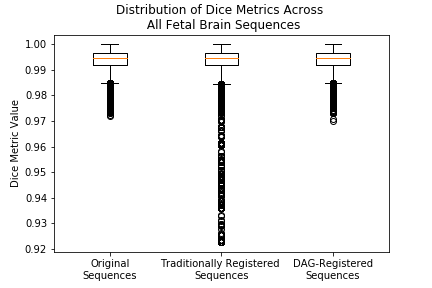
\includegraphics[width=0.5\textwidth]{6/figures/fetal-brain-dice-box.png}
\caption{Boxplots of the values of all Dice matrices for the original sequences, the traditionally registered sequences, and the DAG-registered sequences for the fetal-brain images.}
\label{fig:fetal-brain-dice-box}
\end{figure}

\begin{figure}
\centering
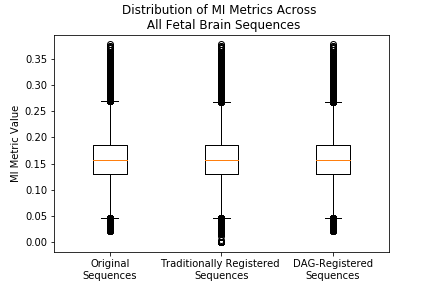
\includegraphics[width=0.5\textwidth]{6/figures/fetal-brain-mi-box.png}
\caption{Boxplots of the values of all MI matrices for the original sequences, the traditionally registered sequences, and the DAG-registered sequences for the fetal brain images.}
\label{fig:fetal-brain-mi-box}
\end{figure}

\begin{table}[]
\centering
\caption{The number of subjects whose sequences of types $S_1$ and $S_2$ had different MI distributions.}
\label{tab:fetal-brain-mi-kstest}
\begin{tabular}{|c|c|c|c|}
\hline
\textbf{\begin{tabular}[c]{@{}c@{}}\# Sequences \\ Type 1 ($S_1$)\end{tabular}} &
  \textbf{\begin{tabular}[c]{@{}c@{}}\# Sequences \\ Type 2 ($S_2$)\end{tabular}} &
  \textbf{\begin{tabular}[c]{@{}c@{}}\# Sequences \\ p \textless 0.05\end{tabular}} &
  \textbf{\begin{tabular}[c]{@{}c@{}}\# Sequences \\ p \textless 0.005\end{tabular}} \\ \hline
Original                                                            & \begin{tabular}[c]{@{}c@{}}Traditionally\\ Registered\end{tabular} & 13 & 10 \\ \hline
Original                                                            & \begin{tabular}[c]{@{}c@{}}DAG\\ Registered\end{tabular}           & 12 & 9 \\ \hline
\begin{tabular}[c]{@{}c@{}}Traditionally \\ Registered\end{tabular} & \begin{tabular}[c]{@{}c@{}}DAG\\ Registered\end{tabular}           & 14 & 9  \\ \hline
\end{tabular}
\end{table}

\subsection{Placenta}

\subsubsection{Volume Registration: Power Thresholds}

\begin{figure}[t]
	\centering
	\begin{subfigure}{0.4\textwidth}
		\centering
		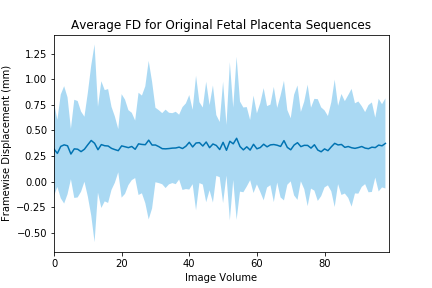
\includegraphics[width=1.0\textwidth]{6/figures/fetal-placenta-bold-fd-150.png}
		\caption{FD of Original Sequences.}
	\end{subfigure}
	\hspace{0.05\textwidth}
	\begin{subfigure}{0.4\textwidth}
		\centering
		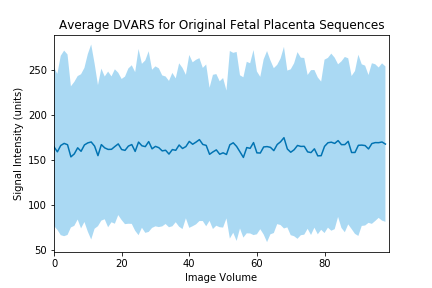
\includegraphics[width=1.0\textwidth]{6/figures/fetal-placenta-bold-dvars-150.png}
		\caption{DVARS of Original Sequences.}
	\end{subfigure}
	
	\begin{subfigure}{0.4\textwidth}
		\centering
		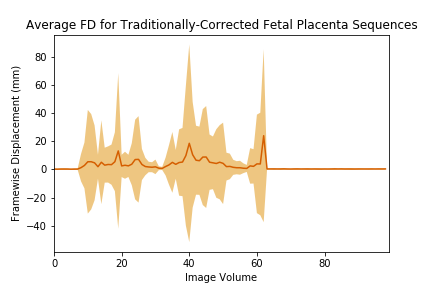
\includegraphics[width=1.0\textwidth]{6/figures/fetal-placenta-trad-fd-150.png}
		\caption{FD of Traditionally Registered Sequences.}
	\end{subfigure}
	\hspace{0.05\textwidth}
	\begin{subfigure}{0.4\textwidth}
		\centering
		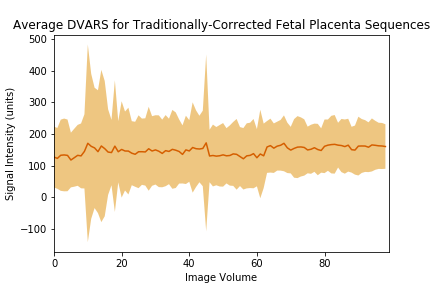
\includegraphics[width=1.0\textwidth]{6/figures/fetal-placenta-trad-dvars-150.png}
		\caption{DVARS of Traditionally Registered Sequences.}
	\end{subfigure}
	
	\begin{subfigure}{0.4\textwidth}
		\centering
		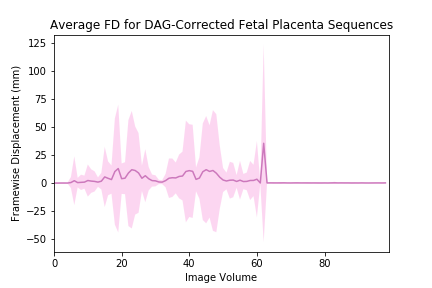
\includegraphics[width=1.0\textwidth]{6/figures/fetal-placenta-dag-fd-150.png}
		\caption{FD of DAG-Registered Sequences.}
	\end{subfigure}
	\hspace{0.05\textwidth}
	\begin{subfigure}{0.4\textwidth}
		\centering
		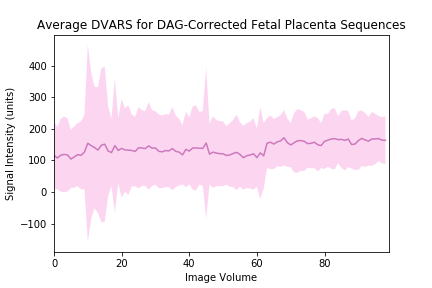
\includegraphics[width=1.0\textwidth]{6/figures/fetal-placenta-dag-dvars-150.png}
		\caption{DVARS of DAG-Registered Sequences.}
	\end{subfigure}
\caption{The means and standard deviations of the FD and DVARS metrics for all placenta images both before and after registration.}
\label{fig:fetal-placenta-power-dists}
\end{figure}

\begin{table}[]
\centering
\caption{The number and percentage of image volumes across all sequences in the fetal placenta image data set which meet the usability thresholds of FD \textless 0.2 mm and DVARS \textless 2.5\%.}
\label{tab:fetal-placenta-power-thresh}
\begin{tabular}{|c|c|c|c|}
\hline
\textbf{Threshold Met} &
  \textbf{\begin{tabular}[c]{@{}c@{}}Original\\  Sequences\end{tabular}} &
  \textbf{\begin{tabular}[c]{@{}c@{}}Traditionally Registered \\ Sequences\end{tabular}} &
  \textbf{\begin{tabular}[c]{@{}c@{}}DAG-Registered \\ Sequences\end{tabular}} \\ \hline
FD (count)    & 10017  & 4113   & 4005   \\ \hline
DVARS (count) & 17     & 1056   & 1624   \\ \hline
Both (count)  & 17     & 599    & 996    \\ \hline
FD (\%)       & 43.646 & 44.245 & 45.020 \\ \hline
DVARS(\%)     & 0.170  & 11.36  & 18.255 \\ \hline
Both (\%)     & 0.170  & 6.444  & 11.196 \\ \hline
\end{tabular}
\end{table}

Table \ref{tab:fetal-placenta-power-thresh} contains the number and percentages of image volumes from the whole neonatal cohort which meet the FD and DVARS thresholds. The total number of image volumes in across the original sequences was 10017, the traditionally registered images was 9296, and the DAG-registered images was 8896.

\subsubsection{Volume Registration: Sequence Duration Motion}

\begin{figure}
\centering
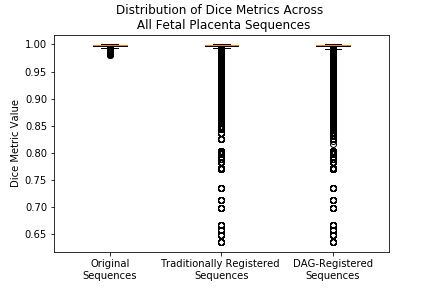
\includegraphics[width=0.5\textwidth]{6/figures/fetal-placenta-dice-box.png}
\caption{Boxplots of the values of all Dice matrices for the original sequences, the traditionally registered sequences, and the DAG-registered sequences for the placenta images.}
\label{fig:fetal-placenta-dice-box}
\end{figure}

\begin{figure}
\centering
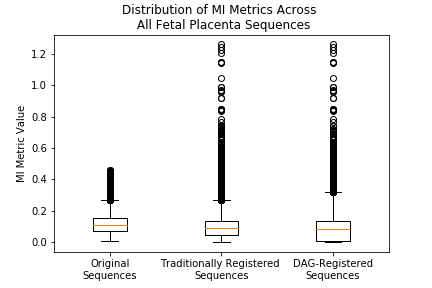
\includegraphics[width=0.5\textwidth]{6/figures/fetal-placenta-mi-box.png}
\caption{Boxplots of the values of all MI matrices for the original sequences, the traditionally registered sequences, and the DAG-registered sequences for the placenta images.}
\label{fig:fetal-placenta-mi-box}
\end{figure}

\section{Characterizing Motion}

\subsection{Age Groups}

\begin{figure}[t]
	\centering
	\begin{subfigure}{0.49\textwidth}
		\centering
		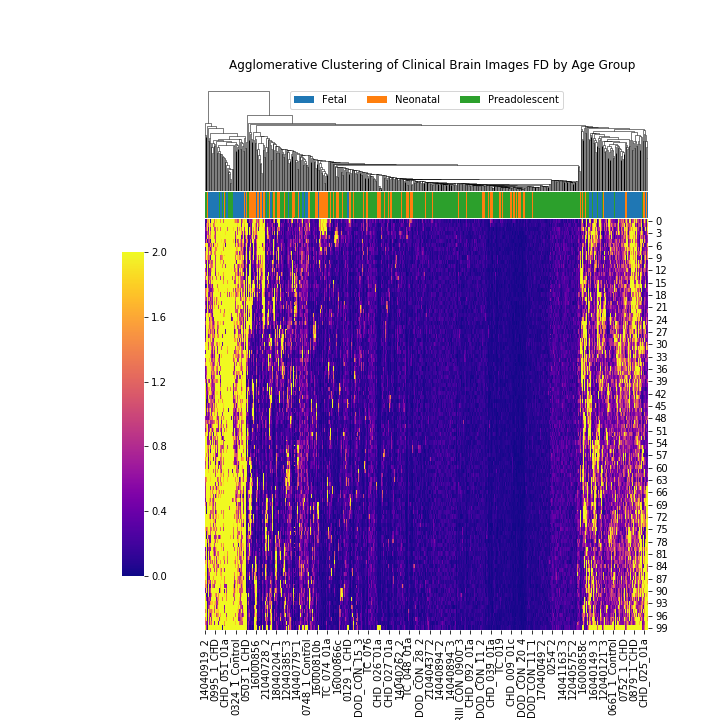
\includegraphics[width=1.0\textwidth]{6/figures/agegroup-bold-fd-sns-agg.png}
		\caption{FD}
	\end{subfigure}
	\begin{subfigure}{0.49\textwidth}
		\centering
		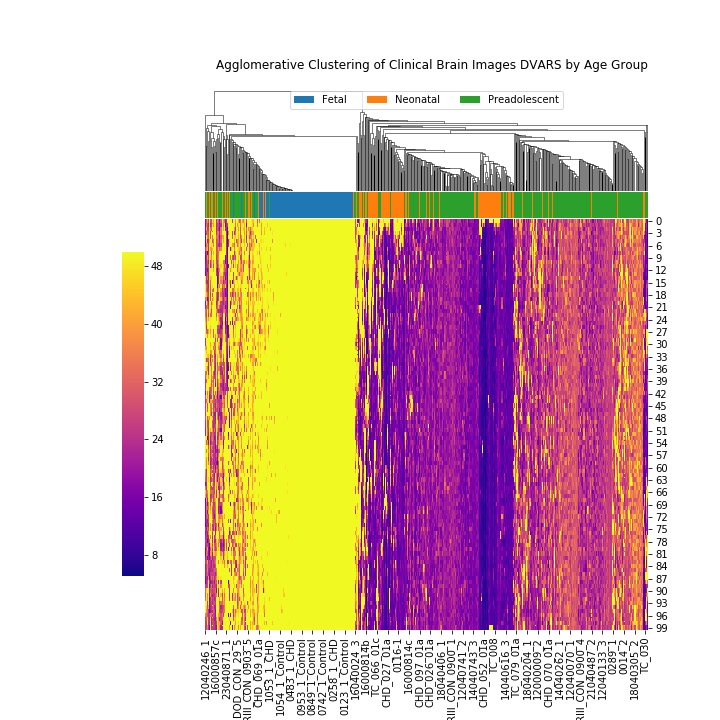
\includegraphics[width=1.0\textwidth]{6/figures/agegroup-bold-dvars-sns-agg.png}
		\caption{DVARS}
	\end{subfigure}
	
	\begin{subfigure}{0.49\textwidth}
		\centering
		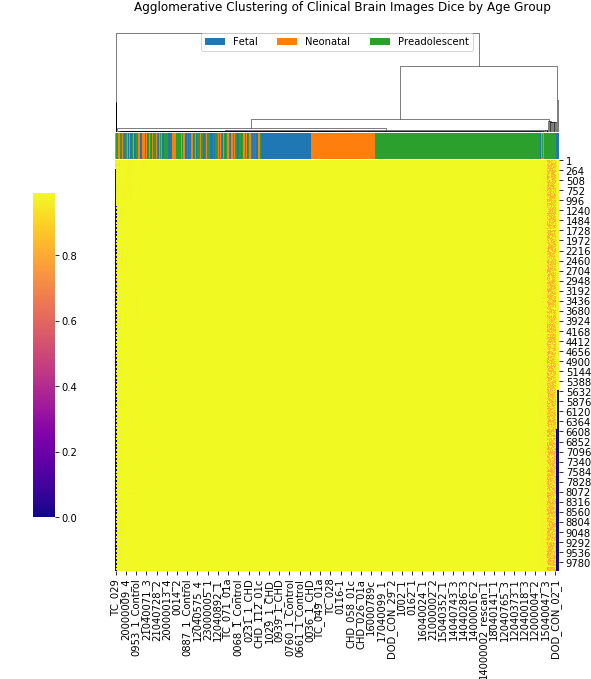
\includegraphics[width=1.0\textwidth]{6/figures/agegroup-bold-dice-sns-agg.png}
		\caption{Dice}
	\end{subfigure}
	\begin{subfigure}{0.49\textwidth}
		\centering
		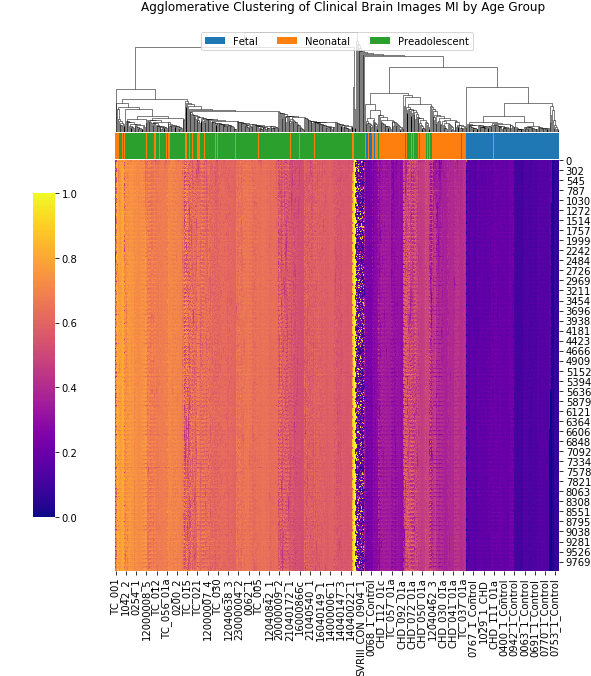
\includegraphics[width=1.0\textwidth]{6/figures/agegroup-bold-mi-sns-agg.png}
		\caption{MI}
	\end{subfigure}
\caption{The preadolescent, neonatal, and fetal images clustered by each metric using agglomerative clustering and labeled by age group.}
\label{fig:mochar-ages-sns-agg}
\end{figure}

\clearpage

\subsection{CHD and Control}

\begin{figure}[t]
	\centering
	\begin{subfigure}{0.49\textwidth}
		\centering
		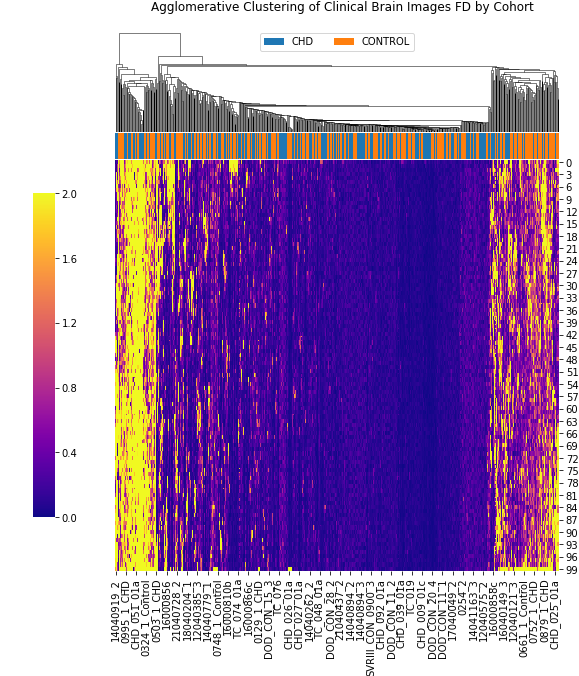
\includegraphics[width=1.0\textwidth]{6/figures/cohort-bold-fd-sns-agg.png}
		\caption{FD}
	\end{subfigure}
	\begin{subfigure}{0.49\textwidth}
		\centering
		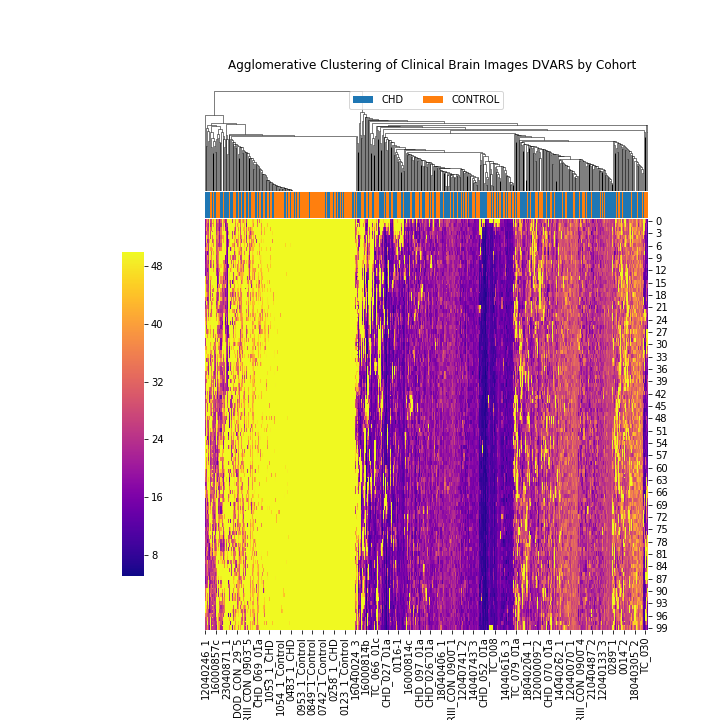
\includegraphics[width=1.0\textwidth]{6/figures/cohort-bold-dvars-sns-agg.png}
		\caption{DVARS}
	\end{subfigure}
	
	\begin{subfigure}{0.49\textwidth}
		\centering
		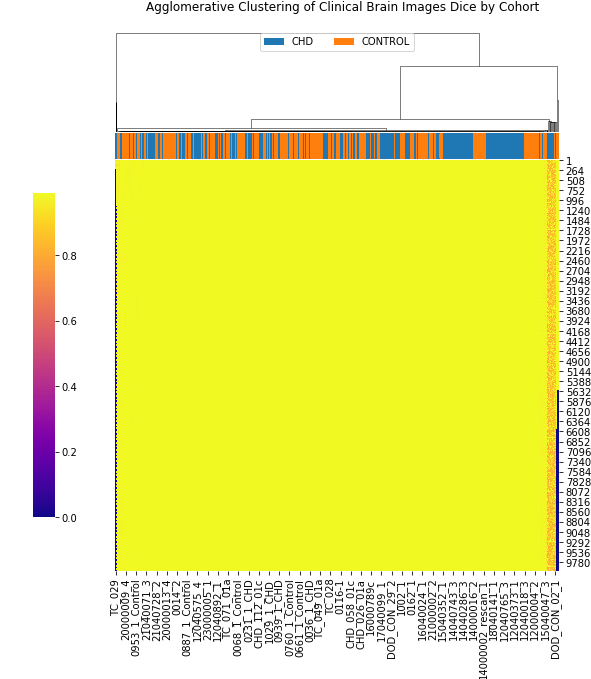
\includegraphics[width=1.0\textwidth]{6/figures/cohort-bold-dice-sns-agg.png}
		\caption{Dice}
	\end{subfigure}
	\begin{subfigure}{0.49\textwidth}
		\centering
		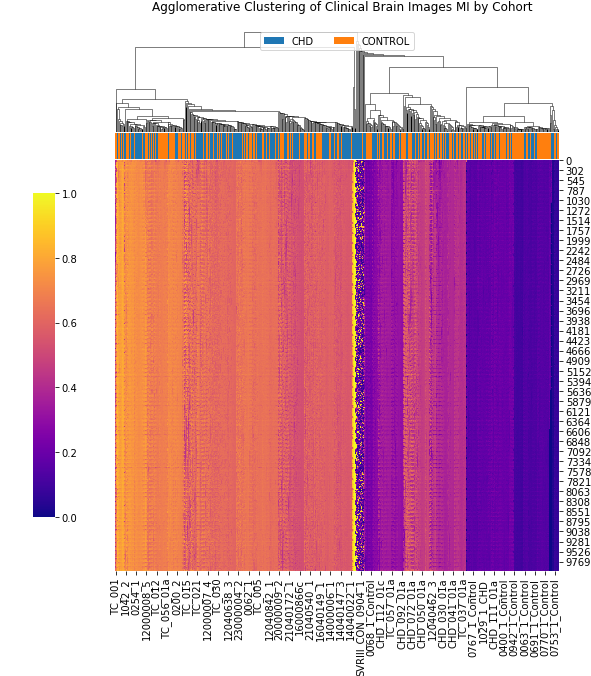
\includegraphics[width=1.0\textwidth]{6/figures/cohort-bold-mi-sns-agg.png}
		\caption{MI}
	\end{subfigure}
\caption{The preadolescent, neonatal, and fetal images clustered by each metric using agglomerative clustering and labeled by CHD/Control status.}
\label{fig:mochar-cohorts-sns-agg}
\end{figure}